\documentclass[a4paper, 12pt]{article}

\usepackage{xspace}
\usepackage{graphicx}
\usepackage{sidecap}
\usepackage{float}
\usepackage{listings}
\usepackage{xcolor}

\colorlet{punct}{red!60!black}
\definecolor{delim}{RGB}{20,105,176}
\colorlet{numb}{magenta!60!black}

\lstdefinelanguage{json}{
    basicstyle=\footnotesize\ttfamily,
    showstringspaces=false,
    breaklines=true,
    literate=
     *{0}{{{\color{numb}0}}}{1}
      {1}{{{\color{numb}1}}}{1}
      {2}{{{\color{numb}2}}}{1}
      {3}{{{\color{numb}3}}}{1}
      {4}{{{\color{numb}4}}}{1}
      {5}{{{\color{numb}5}}}{1}
      {6}{{{\color{numb}6}}}{1}
      {7}{{{\color{numb}7}}}{1}
      {8}{{{\color{numb}8}}}{1}
      {9}{{{\color{numb}9}}}{1}
      {:}{{{\color{punct}{:}}}}{1}
      {,}{{{\color{punct}{,}}}}{1}
      {\{}{{{\color{delim}{\{}}}}{1}
      {\}}{{{\color{delim}{\}}}}}{1}
      {[}{{{\color{delim}{[}}}}{1}
      {]}{{{\color{delim}{]}}}}{1},
}

\begin{document}

\title{Hestia Marketplace Architecture and Design}
\author{Andrew Lalis}
\date{Last Updated: \today}
\maketitle

\tableofcontents
\newpage

\part{Introduction and Background}
	The Hestia Web App is a method by which users can interact with their local Hestia \emph{controllers}, to manipulate certain \emph{devices} in their home. In order for the controller to be able to send the proper commands to such devices, it is imperative that the user install the device's required \emph{plugin}.

	A plugin is a collection of python scripts and configuration files that enables the controller to interact with any IP-enabled device on its local network. To make it easier for users to ensure their devices work without hassle, the \emph{Plugin Marketplace} will provide access to a database of plugins. The marketplace will provide a REST API to let the Web App query plugins and to let plugin developers upload their work.

	From the developer's perspective, a plugin is much more than simply a file folder, and as such, information such as the date of creation, author, and a description need to also be stored so that users can easily understand the contents and purpose of a plugin without needing to dissect any source code.

\part{Architecture and Database Design}
	The main focus of this section will be on the tables needed to store all the information relevant to a plugin. This will consist of a list of attributes that describe a plugin, and any needed auxiliary tables for storing other information in a way that wastes as little space as possible.

	\section{General Architecture}
		In the most general sense, the purpose of the plugin marketplace is to accept requests for plugins, their metadata, or their files. Therefore, the marketplace is designed around the use of REST endpoints to allow users to interact with a privately managed database.

		\begin{figure}[H]
			\caption{A diagram representing the marketplace architecture.}
			\centering
				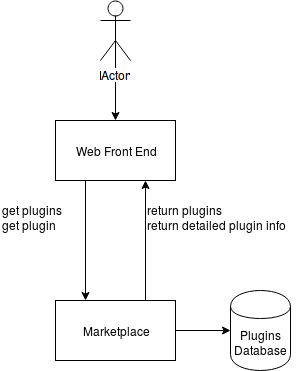
\includegraphics[width=0.5\textwidth]{img/MarketplaceArchitecture.png}
		\end{figure}

	\section{Tables}
		As mentioned before, the most important table in the database is the \textbf{Plugins} table, whose attributes are defined in detail in the following list.

		\begin{itemize}
			\item \emph{id} - A globally unique identification string which can be used to reference this plugin.
			\item \emph{name} - The name of the plugin, as it will appear in lists when users wish to browse the list of plugins.
			\item \emph{author\_id} - The unique authenticated id of the user who uploaded the plugin.
			\item \emph{created\_date} - The date on which the plugin was first uploaded.
			\item \emph{last\_edited\_date} - The date of the most recent update to the plugin.
			\item \emph{version} - A string of numbers representing the current version of the plugin. This is up to the author's discretion.
			\item \emph{description\_short} - A short and concise description, less than 100 characters, which can be displayed in menus to give users a hint as to what the plugin does.
			\item \emph{description\_long} - A much more detailed description of the plugin, which provides detailed instructions for use of the plugin, or other relevant details that the author thinks the users should know.
			\item \emph{up\_goats} - Up-Goats represent the number of users who cast a positive vote for the plugin, meaning that they believe it is valuable and useful.
			\item \emph{down\_goats} - Down-Goats are the opposite of Up-Goats, and count the number of users who voted negatively for the plugin.
		\end{itemize}

		Additionally, some other tables are needed to provide auxiliary information to make the user experience more enjoyable. These are defined below.

		The \textbf{Tags} table holds many tags, which are can be applied to many plugins to group them into related categories.

		\begin{itemize}
			\item \emph{name} - A unique string which represents a tag, which can be applied to a plugin to give it some extra meaning.
			\item \emph{description} - A short description of the tag, or an embellishment of its meaning.
		\end{itemize}

		In order to manifest the \emph{many-to-many} relationship between tags and plugins, a third table, \textbf{PluginTags}, is needed to pair the two together.

		\begin{itemize}
			\item \emph{plugin\_id} - The global id of the plugin paired with a tag.
			\item \emph{tag\_name} - The unique name of a tag which is paired to the above plugin.
		\end{itemize}

	\section{File Storage}
		Because the core of each plugin is a collection of files, these will need to be stored in or alongside the database. In order to keep the files synchronized with the contents of the actual relational database, a \textbf{plugins} folder will contain many \verb|.zip| files, each named according the the globally unique id number of the plugin they represent.

\part{REST API}
	This section contains the API documentation for the HTTP methods used to interact with the server, and defines the syntax for making requests, as well as what responses should be expected when requests are made, valid or not.

	\section{GET plugins}
		Returns some basic information about all available plugins, while omitting more specific information like \emph{description\_long}.

		\subsection{Syntax}
			\verb|GET <URL>/plugins|

		\subsection{Responses}
			\subsubsection{Success}
				In the likely event that the server can retrieve the list of plugins, it will return a \verb|JSON| object containing all the plugins' metadata. The structure of that object is defined below.

				\lstinputlisting[language=json]{code/get_plugins_example.json}

			\subsubsection{Server Error}
				Because no parameters are required, any error, given a proper \verb|URL|, is the fault of the server, and as such, a \verb|500 Internal Error| message will be returned.

	\section{GET a plugin's metadata}
		Returns more detailed information about a specific plugin, including the \emph{description\_long}.

		\subsection{Syntax}
			\verb|GET <URL>/plugin/<PLUGIN_ID>|; \footnotesize{Where \verb|PLUGIN_ID| is the unique id of the plugin.}

		\subsection{Responses}
			\subsubsection{Success}
				If the server successfully finds a plugin with the id specified in the URL, then it will return a JSON object with the structure shown below.

				\lstinputlisting[language=json]{code/get_plugin_example.json}

			\subsubsection{Plugin Not Found}
				If the id specified in the URL does not refer to any existing plugin, then a \verb|404 Not Found| error message will be returned.

			\subsubsection{Server Error}
				If the server fails to retrieve information for a plugin which may or may not exist, or if the server fails in some other way, on its own fault, it will return \verb|500 Internal Error|.

	\section{GET a plugin's zipped files}
		Returns the \verb|.zip| file associated with a plugin whose id is specified in the request.

		\subsection{Syntax}
			\verb|GET <URL>/plugin/<PLUGIN_ID>/files|; \footnotesize{Where \verb|PLUGIN_ID| is the unique id of the plugin.}

		\subsection{Responses}
			\subsubsection{Success}
				If the plugin specified by the given id exists, then the server will return 

\end{document}